\documentclass[11pt]{article}

\usepackage[T1]{fontenc}      % needed for \DJ (Đ in "Đoković")
\usepackage[margin=1in]{geometry}
\usepackage{amsmath,amssymb,amsthm,mathtools}
\usepackage{longtable}
\usepackage{graphicx}
\usepackage{hyperref}

\newtheorem{theorem}{Theorem}
\newtheorem{lemma}{Lemma}
\newtheorem{corollary}{Corollary}
\newtheorem{remark}{Remark}

\newcommand{\F}{\mathbb F}
\newcommand{\Z}{\mathbb Z}
\newcommand{\J}{J}
\newcommand{\I}{I}
\newcommand{\Rcal}{\mathcal R}

\title{A Paley--II analogue of the Scarpis--\DJ okovi\'c construction\\
       for prime powers \(q\equiv 1\pmod 4\)}
% Edit author/affiliation as appropriate before submission.
\author{Jeffery Kline}
\date{\today}

\begin{document}

\maketitle

\begin{abstract}
A Hadamard matrix of order \(m\) is a \(\{1,-1\}\)-matrix \(H\) with
\(HH^{T}=mI_{m}\).  Scarpis (1898) showed that for a prime
\(p\equiv 3\pmod 4\) a Hadamard matrix of order \(p+1\) can be lifted to
one of order \(p(p+1)\), and \DJ okovi\'c extended the lift to all prime
powers \(q\equiv 3\pmod 4\), asking for the analogous procedure for
\(q\equiv 1\pmod 4\).  That case was settled by Farouk and Wang (2020),
who lift an input Hadamard matrix of order \(2(q+1)\), subject to
eligibility conditions, to one of order \(2q(q+1)\), verifying
orthogonality by row-pair counting arguments in which the key inner
products are imported from the Hadamard property of the input matrix.
This note contributes a different method, not a new existence result.
Both routes are constructive; the difference is procedure versus
formula: their lift takes choices --- an input matrix and a bijection
--- that can change the output, while the matrix here is given by a
choice-free closed form, one matrix for each \(q\).  There is no input
matrix: the finite bands are given entrywise in
closed form by the quadratic character on \(\F_q\) composed with the
\(2\times 2\) Paley--II replacement blocks, and the Hadamard property
is proved by four block-Gram identities computed directly from
character sums.  The printed outputs differ as well: at \(q=5\) our matrix is
not Hadamard-equivalent to the order-\(60\) example printed by Farouk
and Wang, although it need not differ from every output of their
procedure (Remark~\ref{rem:alpha5}).

We then ask what the construction actually requires.  Replacing the
character by a function \(\delta\colon G\to\{0,\pm1\}\) with
\(\delta(0)=0\) on a finite abelian group \(G\) of order \(n\), and the
shift by an arbitrary array \(T\), the resulting matrix is Hadamard
\emph{if and only if} \(\delta\) is of Paley type and \(T\) is a
\((G,n;1)\)-difference matrix.  The sufficiency half is known in greater
generality, in the Butson setting and without commutativity, from Seberry
and from Nu\~nez Ponasso; what is new here is the converse, that the two
conditions are forced.  They separate the sign
pattern from the shift array and account for the shape of the family:
the first makes \(\{z:\delta(z)=1\}\) a regular partial difference set
with the Paley parameters, forcing \(n\equiv1\pmod4\); the second
yields \(n-1\) mutually orthogonal Latin squares, so an instance on a
group of non-prime-power order would produce a projective plane of
non-prime-power order.

A second reading of the same matrix is arithmetic rather than
combinatorial.  The Paley--II blocks are the real \(2\times2\)
representation of the Gaussian units, and through it the construction
factors through a Butson matrix \(\Gamma\in BH\bigl(q(q+1),4\bigr)\) of
half the order whose Turyn double is \(H\).  This locates the note
against a second line in the literature: composing the complex Scarpis
lift of Sargent, Lee and Rushall (2024) with the same doubling gives a
further route to the existence statement, alongside Farouk and Wang,
and \(\Gamma\) is equivalent to one of their outputs.

We also make the family's coverage explicit:
every order \(2q(q+1)\) whose odd part is at most \(3000\) is already
recorded in the
standard tables, and the smallest order lying beyond that audited range,
\(q=81\) (order \(13284=4\cdot 41\cdot 81\)), also follows from a
classical Turyn product using \(T\)-matrices of order \(41\) and
Williamson-type matrices of order \(81=9^{2}\).  We exhibit the
witnessing constructions, identify the smallest
unaudited order, give a second worked example lying beyond the reach of
the elementary screen, and
tabulate, for \(q\le3000\), those orders for which a deliberately
restricted elementary screen supplies no witness, emphasising that these
are \emph{unaudited} rather than open.
\end{abstract}

\section{Introduction}

For a prime power \(q\) let \(\F=\F_q\) and let
\(\chi\colon\F\to\{0,\pm1\}\) be the quadratic character,
\(\chi(0)=0\), \(\chi(x)=1\) for nonzero squares and \(-1\) otherwise.
Paley's two constructions split on the residue of \(q\): for
\(q\equiv 3\pmod 4\) Paley~I gives a Hadamard matrix of order \(q+1\),
and for \(q\equiv 1\pmod 4\) Paley~II gives one of order \(2(q+1)\)
\cite{Paley1933}.

Scarpis \cite{Scarpis1898} showed that for a prime \(p\equiv 3\pmod 4\) a
Hadamard matrix of order \(p+1\) lifts to one of order \(p(p+1)\).
\DJ okovi\'c \cite{Djokovic2016} replaced the prime by an arbitrary prime
power: if \(q\equiv 3\pmod 4\) is a prime power there is a Hadamard
matrix of order \(q(q+1)\); his note closes with the open problem of an
analogous procedure for \(q\equiv 1\pmod 4\).

Because the Paley--II seed has order \(2(q+1)\), the natural
Scarpis-type target in the \(q\equiv 1\pmod 4\) case is
\[
        q\cdot 2(q+1)=2q(q+1).
\]
We construct such a matrix directly from \(\chi\).  Throughout, \(q\equiv
1\pmod 4\) is a prime power, so \(\chi(-1)=1\); this is the only place
the residue class is used, and it is exactly what fails for
\(q\equiv 3\pmod 4\).

The existence of Hadamard matrices of order \(2q(q+1)\) for prime powers
\(q\equiv1\pmod4\) is due to Farouk and Wang \cite{FaroukWang2020}; the
contribution of this note is the method of
construction and proof.  Farouk and Wang obtain the matrix as the output
of a lifting procedure applied to an input Hadamard matrix of order
\(2(q+1)\) meeting certain eligibility conditions, and their verification
proceeds row pair by row pair, by counting arguments in which the key
inner-product values are imported from the Hadamard property of the
input matrix.  Here there is no input matrix: the finite bands are
written entrywise in the closed form \(\psi(\chi(y-x-t))\), and the
Hadamard property follows from four block-Gram identities whose
ingredients are computed directly from the quadratic character --- the
sums \eqref{eq:rowsum} and \(\sum_{z}\chi(z(z-d))=-1\), together with
the block identity \(P+ZR=0\).  The proof is thus self-contained at the
level of character sums, and the single place where the residue class
enters, \(\chi(-1)=1\), is isolated.  A secondary contribution is the
coverage analysis of Appendix~\ref{app:coverage}, which has no
counterpart in \cite{FaroukWang2020}: it locates the initial range
against audited tables of known Hadamard orders and applies a restricted
elementary screen beyond that range.

\section{The Paley--II blocks}

Put
\[
P=\begin{pmatrix}1&1\\ 1&-1\end{pmatrix},\quad
Z=\begin{pmatrix}1&-1\\ -1&-1\end{pmatrix},\quad
R=\begin{pmatrix}0&-1\\ 1&0\end{pmatrix},
\]
and let \(\psi\colon\{0,\pm1\}\to\{\pm1\}^{2\times2}\) be
\(\psi(0)=Z\), \(\psi(1)=P\), \(\psi(-1)=-P\); these are the Paley--II
replacement blocks, and \(ZR=-P\).  Write \(\Rcal=\J_q\otimes I_2\),
where \(\J_q\) is the \(q\times q\) all-ones matrix.  We use repeatedly
\[
        \sum_{u\in\F}\psi(\chi(u))=Z,
        \tag{2.1}\label{eq:rowsum}
\]
which holds because the nonzero squares and non-squares are equinumerous,
and the character sum
\[
        \sum_{z\in\F}\chi\bigl(z(z-d)\bigr)=-1\qquad(d\neq0).
        \tag{2.2}\label{eq:charsum}
\]
For the latter, the term \(z=0\) contributes \(\chi(0)=0\), while for
\(z\neq0\) we have \(z(z-d)=z^{2}\bigl(1-dz^{-1}\bigr)\) with
\(\chi(z^{2})=1\); as \(z\) runs over \(\F^{\times}\) the element
\(u=1-dz^{-1}\) runs over \(\F\setminus\{1\}\), so the sum equals
\(\sum_{u\neq1}\chi(u)=-\chi(1)=-1\) because \(\sum_{u\in\F}\chi(u)=0\).

\section{The construction}

For \(t\in\F\) let \(K_t\) be the \(2q\times2q\) matrix with rows and
columns indexed by pairs \((x,a)\), \(x\in\F\), \(a\in\{0,1\}\), whose
\(2\times2\) block in position \((x,y)\) is
\[
        K_t[x,y]=\psi\bigl(\chi(y-x-t)\bigr).
\]

\begin{lemma}\label{lem:self}
For every \(t\in\F\), \(\;K_tK_t^{T}=2(q+1)I_{2q}-2\Rcal.\)
\end{lemma}

\begin{proof}
The \((x,x')\) block of \(K_tK_t^{T}\), with \(d=x'-x\) and
\(z=y-x-t\), equals \(\sum_{z}\psi(\chi(z))\psi(\chi(z-d))^{T}\).  For
\(d=0\) each summand is \(2I_2\), giving \(2qI_2\).  For \(d\neq0\) the
terms \(z=0\) and \(z=d\) carry opposite skew parts and cancel, using
\(\chi(-d)=\chi(d)\) (here \(\chi(-1)=1\)); for \(z\neq0,d\),
\(\psi(\chi(z))\psi(\chi(z-d))^{T}=2\chi(z)\chi(z-d)I_2\), and
\eqref{eq:charsum} yields \(-2I_2\).  These are the diagonal and
off-diagonal blocks of \(2(q+1)I-2\Rcal\).
\end{proof}

\begin{lemma}\label{lem:cross}
For \(r,s\in\F\),
\[
        \sum_{a\in\F}K_{ar}K_{as}^{T}=
        \begin{cases}
        2q(q+1)I_{2q}-2q\Rcal,&r=s,\\
        2\Rcal,&r\neq s.
        \end{cases}
\]
\end{lemma}

\begin{proof}
The case \(r=s\) is \(q\) copies of Lemma~\ref{lem:self}.  For
\(r\neq s\), in the \((x,x')\) block put \(z=y-x-ar\); the second
argument becomes \(z-(x'-x)+a(r-s)\), which ranges over all of \(\F\)
independently of \(z\) as \(a\) does.  By \eqref{eq:rowsum} each block is
\(Z Z^{T}=2I_2\), i.e.\ the corresponding block of \(2\Rcal\).
\end{proof}

For \(r\in\F\) let \(B_r\) be the \(2q\times2q\) matrix whose row
\((x,a)\) equals row \((r,a)\) of \(K_0\) for every \(x\); thus \(B_r\)
has only two distinct rows.  From Lemma~\ref{lem:self},
\(B_rB_s^{T}=2q\Rcal\) if \(r=s\) and \(-2\Rcal\) if \(r\neq s\).

Form the \(2q\times2q(q+1)\) block rows
\(M_r=\bigl[\,B_r\mid K_{ar}\ (a\in\F)\,\bigr].\)

\begin{lemma}\label{lem:finite}
\(M_rM_s^{T}=2q(q+1)I_{2q}\) if \(r=s\), and \(0\) if \(r\neq s\).
\end{lemma}

\begin{proof}
\(M_rM_s^{T}=B_rB_s^{T}+\sum_aK_{ar}K_{as}^{T}\).  For \(r=s\) the
\(2q\Rcal\) of the border cancels the \(-2q\Rcal\) of
Lemma~\ref{lem:cross}; for \(r\neq s\) the \(-2\Rcal\) cancels the
\(2\Rcal\).
\end{proof}

Let \(C\) be the Paley conference matrix indexed by
\(\{\infty\}\cup\F\), namely \(C_{u,u}=0\),
\(C_{\infty,x}=C_{x,\infty}=1\), \(C_{x,y}=\chi(y-x)\), and let \(S\) be
the order-\(2(q+1)\) Paley--II Hadamard matrix obtained by replacing
\(0,1,-1\) by \(Z,P,-P\).  Delete the two rows of \(S\) indexed by
\(\infty\); in each remaining row repeat the \(\infty\)-column pair
\(q\) times unchanged, and replace each finite column pair by its
product with \(R\), repeated \(q\) times.  This is a
\(2q\times2q(q+1)\) matrix \(M_\infty\).  In both cases the \(q\) copies
of a given column pair are placed \emph{consecutively}, so that a column
pair \(V\) (of size \(2q\times2\)) becomes the \(2q\times2q\) block
\(\J_{1,q}\otimes V=[\,V\mid V\mid\cdots\mid V\,]\).
Thus \(M_\infty\) carries the same column partition as \(M_r\)
above, an initial \(2q\)-wide \(\infty\)-block followed by \(q\) blocks
of width \(2q\) indexed by \(\F\), and for each \(a\in\F\) the
\(a\)-block of \(M_\infty\) occupies the columns that \(K_{ar}\) occupies
in \(M_r\).  This alignment is what the block-by-block summation in
Lemma~\ref{lem:cap} uses; the interleaved reading, in which the copies of
distinct column pairs alternate, does not yield a Hadamard matrix.

\begin{lemma}\label{lem:cap}
\(M_\infty M_\infty^{T}=2q(q+1)I_{2q}\) and \(M_\infty M_r^{T}=0\) for all
\(r\in\F\).
\end{lemma}

\begin{proof}
The first identity holds because \(S\) is Hadamard \cite{Paley1933}, each column pair is
repeated \(q\) times, and right multiplication by \(R\) preserves row
inner products.  For the cross identity, summing a cap row against a row
of \(M_r\) and using \eqref{eq:rowsum} on every \(2q\)-block leaves
\(\bigl(P_\alpha+(\sum_{a}S[e,a]_\alpha)R\bigr)\cdot Z_\beta\); the inner
sum of finite entries of a row of \(S\) is \(Z_\alpha\), and
\(P+ZR=P-P=0\).
\end{proof}

\begin{theorem}\label{thm:main}
Let \(q\equiv1\pmod4\) be a prime power.  Then
\[
        H=\begin{bmatrix}M_\infty\\ M_r\ (r\in\F)\end{bmatrix}
\]
is a Hadamard matrix of order \(2q(q+1)\).
\end{theorem}

\begin{proof}
\(H\) is \(\{1,-1\}\) and square of order \(2q+q\cdot2q=2q(q+1)\).
Lemmas~\ref{lem:finite} and \ref{lem:cap} give
\(HH^{T}=2q(q+1)I\).
\end{proof}

\begin{corollary}
For every prime power \(q\equiv1\pmod4\) there is a Hadamard matrix of
order \(2q(q+1)\); the smallest non-prime instance is \(q=9\), of order
\(180\).
\end{corollary}

The construction has been verified by full Gram computation for all
\(q\le49\) (orders \(60,\dots,4900\), including the extension fields
\(q=9,25,49\)) and by streamed row-orthogonality checks for \(q=81\) and
\(q=125\) (orders \(13284\) and \(31500\)).

\section{Relation to the Farouk--Wang construction}

Theorem~\ref{thm:main} gives, for the \(q\equiv1\pmod4\) case, an
explicit form of the Scarpis-type family that \DJ okovi\'c
\cite{Djokovic2016} asked for.  That family was already constructed by
Farouk and Wang \cite{FaroukWang2020,FaroukWang2022} from the same
order-\(2(q+1)\) Paley--II seed.  This section records how the two
routes differ and where the orders of the family sit relative to the
audited tables of known Hadamard orders.

While Theorem~\ref{thm:main} and \cite[Cor.~2.1]{FaroukWang2020} assert
the same existence result, the routes differ.  Farouk and Wang obtain
the order-\(2q(q+1)\) matrix from a lifting procedure applied to a
Hadamard matrix of order \(2(q+1)\) satisfying the eligibility
conditions of \cite[Lem.~2.2]{FaroukWang2020} --- a formally larger
input class, with Paley~II the only exhibited member --- and verify
orthogonality row pair by row pair through counting arguments (row
sums, balanced sign-pair tallies, and a unique-intersection
computation), importing the key inner-product values from the Hadamard
property of the input matrix.  The present note fixes the Paley--II
seed and writes the finite bands entrywise in the closed form
\(\psi(\chi(y-x-t))\); the Hadamard property follows from four
block-Gram identities in which the corresponding quantities are
computed directly from the character sums \eqref{eq:rowsum} and
\(\sum_{z}\chi(z(z-d))=-1\), together with \(P+ZR=0\) and the
Hadamard property of the Paley--II seed \(S\) (itself a
character-sum identity).  The
correspondence is exact: their unique-intersection index matches the
affine collision \(x+ar=x'+as\) in the substitution step of
Lemma~\ref{lem:cross}, and their imported inner products match the
values that Lemma~\ref{lem:self} derives from
\(\sum_{z}\chi(z(z-d))=-1\).  The devices used for the cap band also
differ: a column permutation arranging balanced sign pairs in
\cite{FaroukWang2020} versus right multiplication by \(R\) here.

\begin{lemma}\label{lem:quadinv}
Let \(M=(m_{ic})\) have all entries of modulus \(1\).  The multiset of
\(\bigl|\sum_cm_{ic}\overline{m_{jc}}m_{kc}\overline{m_{lc}}\bigr|\), taken
over quadruples of distinct rows --- equivalently, the multiset of its
squares --- is unchanged by permuting rows or columns, by multiplying any row
or column by a scalar of modulus \(1\), and by complex conjugation.
\end{lemma}

\begin{proof}
Permuting rows permutes the quadruples and permuting columns permutes the
summands.  Multiplying row \(i\) by \(u\) multiplies every summand by \(u\)
or by \(\bar u\), and multiplying column \(c\) by \(v\) multiplies the
\(c\)-th summand by \(v\bar vv\bar v=|v|^{4}=1\); conjugating \(M\) conjugates
every sum.  No absolute value changes in any case.
\end{proof}

For a \(\{1,-1\}\)-matrix the conjugations are vacuous and the admissible
scalars are \(\pm1\), which is the form used below and in
Remark~\ref{rem:q9}; the column profile of \(M\) is the row profile of
\(M^{T}\).  The
two constructions do not merely present the same matrix differently: at
\(q=5\) the matrix of
Theorem~\ref{thm:main} is not Hadamard-equivalent to the order-\(60\)
example printed in the appendix of \cite{FaroukWang2020} --- the
multiset of absolute row-quadruple correlations
\(\bigl|\sum_{c}h_{ic}h_{jc}h_{kc}h_{lc}\bigr|\), an invariant of
Hadamard equivalence, differs for the two matrices
(Figure~\ref{fig:q5sbs}).  Since Farouk and
Wang note that their output may vary with the choice of bijection
\(\alpha\), the matrix of Theorem~\ref{thm:main} may still be equivalent to
some other output of their procedure; see Remark~\ref{rem:alpha5}.

\begin{remark}[unrefereed computational report]\label{rem:alpha5}
The following is \emph{not} a claim of this note.  It was produced by
automated agents, has been checked here only by re-running the computation,
and has not been refereed; we record it because it bears directly on the
paragraph above.  The report is that at \(q=5\) the matrix of
Theorem~\ref{thm:main} \emph{is} Hadamard-equivalent to an output of the
Farouk--Wang procedure --- to \(\Psi_{5,\alpha}(P'_5)\) for \(\alpha\) any of
the twenty affine bijections \(k\mapsto ak+b\) of \(\F_5\) --- by an explicit
signed row and column permutation, exhibited and checked by exact integer
identity in \texttt{code/alpha\_family.py}.  If it is right, the inequivalence
recorded above separates the matrix of Theorem~\ref{thm:main} from the
particular representative printed in \cite{FaroukWang2020}, not from the
family \(\Psi_{5,\alpha}\); the same computation reports that three of the
four profiles arising in that family do differ from ours, so the matrix is
equivalent to some outputs and inequivalent to others.  Two caveats are
essential.  It covers \(q=5\) alone.  And it rests on a reading of
\cite[Steps 4--7]{FaroukWang2020} that required correcting the permutation
displayed in the proof of their Lemma 2.2(2), which at \(q=5\) does not
satisfy their own condition; their Theorem 2.2 and Corollary 2.1 are
unaffected.  Independent verification is wanted.
\end{remark}

\begin{figure}[t]
\centering
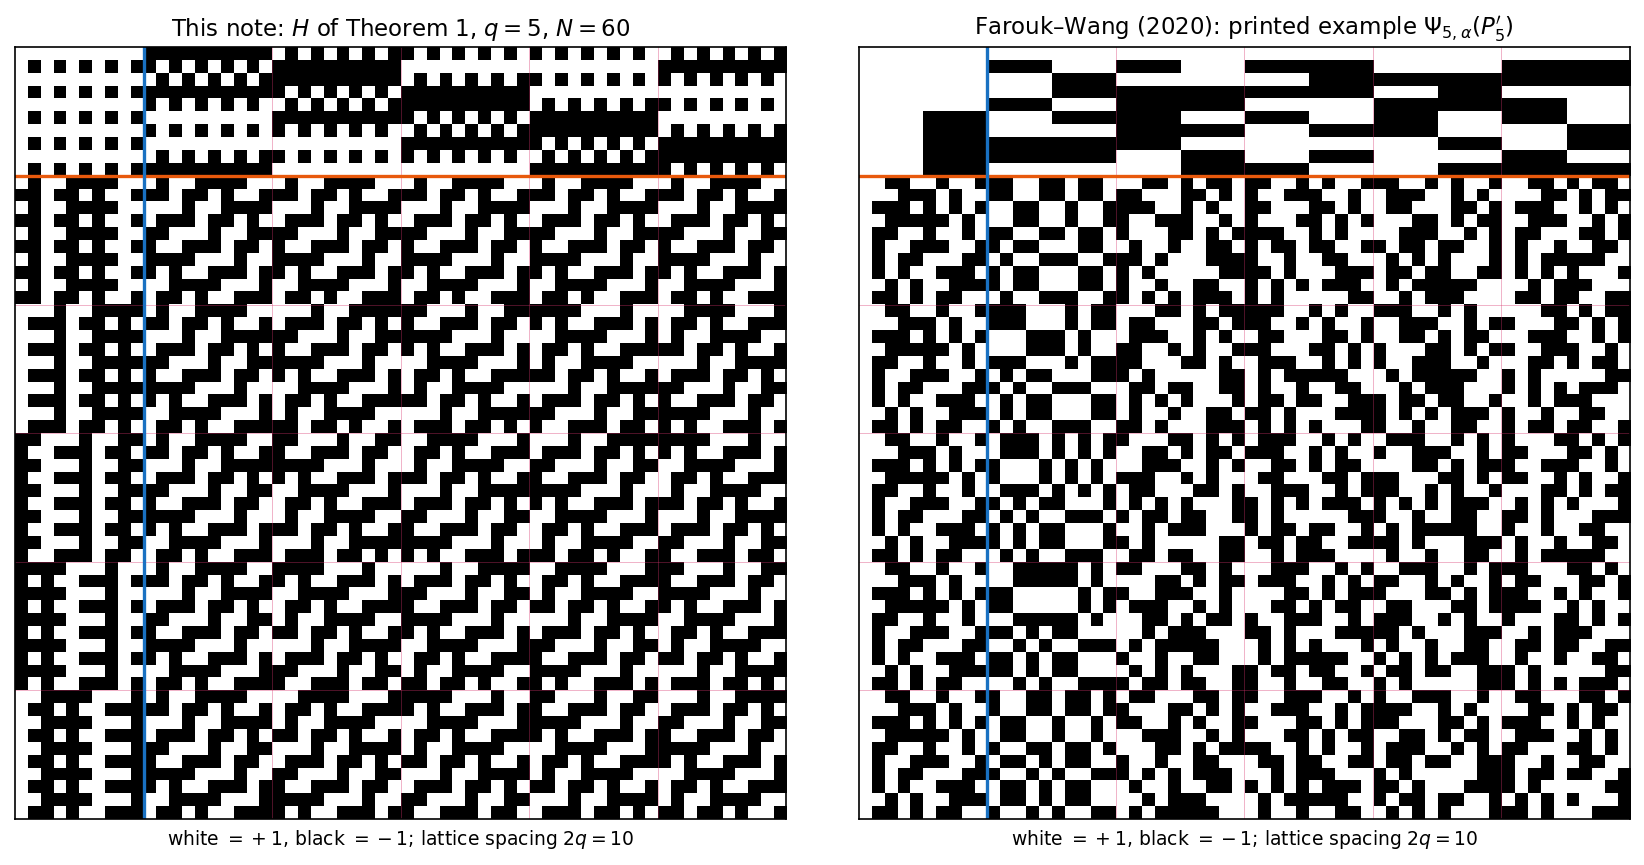
\includegraphics[width=\textwidth]{images/q5_side_by_side}
\caption{The two constructions at \(q=5\) (order \(60\); white
\(=+1\), black \(=-1\); lattice spacing \(2q=10\)).  Left: the matrix
of Theorem~\ref{thm:main} --- the cap band \(M_\infty\) above the
orange separator is a family of period-two column patterns, and the
finite bands \(M_r\) carry the diagonal texture of the shifts
\(\psi(\chi(y-x-ar))\).  Right: the order-\(60\) example
\(\Psi_{5,\alpha}(P_5')\) printed in the appendix of
\cite{FaroukWang2020}, whose top band is a coarse tiling (its border
block consists of four constant \(5\times5\) quadrants) and whose
finite bands show no diagonal structure.  The two matrices are
Hadamard-inequivalent: over the \(\binom{60}{4}=487{,}635\) row
quadruples, the right matrix attains
\(\bigl|\sum_{c}h_{ic}h_{jc}h_{kc}h_{lc}\bigr|=28\) on \(400\)
quadruples, the left on none, and this multiset is invariant under row
and column permutations and negations (and the comparison fails in
both orientations, covering the transpose convention as well).  This
separates the printed representative only: outputs of the Farouk--Wang
procedure for other choices of \(\alpha\) are not addressed.}
\label{fig:q5sbs}
\end{figure}

Since \(q\equiv1\pmod4\), the \(2\)-adic valuation of the order is
exactly \(2\):
\[
        2q(q+1)=4\cdot q\cdot\tfrac{q+1}{2},
        \qquad q\ \text{and}\ \tfrac{q+1}{2}\ \text{both odd.}
        \tag{4.1}\label{eq:fourodd}
\]
Thus every order is \(4\times(\text{odd})\), so it is never a Kronecker
product of two smaller Hadamard matrices, and its odd part
\(q(q+1)/2\) is always composite.  That last fact is a structural
description and not an exclusion: of the \(195\) odd \(m\le2999\) for
which \cite{CatiPasechnik2024} records no Hadamard matrix of order
\(4m\), fully \(71\) are composite, so compositeness of the odd part does
not by itself keep an order off the open list.  Whether the family meets
that list has to be checked value by value, and
Appendix~\ref{app:audit} does so for the whole range \(q\le73\).
A second and more useful consequence is that \eqref{eq:fourodd} has the form needed
for Turyn's construction: when \(T\)-matrices of order \(t\) and
Williamson-type matrices of order \(w\) are available, one obtains a
Hadamard matrix of order \(4tw\)
\cite{Turyn1974,SeberryYamada1992}, and here \(\{t,w\}=\{q,(q+1)/2\}\).
The coverage analysis of Appendix~\ref{app:coverage} makes both points
quantitative: all orders with odd part \(\le 3000\) are recorded in the
standard tables, the first order beyond that range is covered by such a
Turyn product, and a restricted screen beyond the audited range records
exactly which orders it does and does not cover.  Failure of that screen is
not a claim that an order is open.

\section{What the construction needs}\label{sec:char}

Theorem~\ref{thm:main} is stated over \(\F_q\), but the field enters the
proofs of Lemmas~\ref{lem:self}--\ref{lem:cap} in only two ways: through the
character sums attached to \(\chi\), and, at exactly one line in the proof of
Lemma~\ref{lem:cross}, through the fact that \(a\mapsto a(r-s)\) is a
bijection of \(\F\) when \(r\neq s\).  This section replaces each of the two
by an abstract hypothesis and shows that the resulting pair of conditions is
not merely sufficient but necessary.  The conclusion is a clean division of
labour --- one condition on the sign pattern, one on the shift array --- and,
through the second condition, an explanation of why the family is confined to
prime powers.

Let \(G\) be a finite abelian group, written additively, with \(|G|=n\).
Replace \(\chi\) by a function \(\delta\colon G\to\{0,\pm1\}\) with
\(\delta(0)=0\), and replace the shift \(ar\) by an arbitrary array
\(T\colon G\times G\to G\).  Put
\[
        K_t[x,y]=\psi\bigl(\delta(y-x-t)\bigr)\qquad(x,y\in G),
\]
let \(B_r\) be the \(2n\times2n\) matrix each of whose rows \((x,\alpha)\)
equals row \((r,\alpha)\) of \(K_0\), and set
\[
        M_r=\bigl[\,B_r\mid K_{T(r,a)}\ (a\in G)\,\bigr],\qquad r\in G .
\]
Let \(C\) be indexed by \(\{\infty\}\cup G\) with \(C_{u,u}=0\),
\(C_{\infty,x}=C_{x,\infty}=1\), \(C_{x,y}=\delta(y-x)\), let \(S\) be its
\(\psi\)-replacement, and let \(M_\infty\) be built from \(S\) exactly as in
\S3.  Write
\[
        H(G,\delta,T)=\begin{bmatrix}M_\infty\\ M_r\ (r\in G)\end{bmatrix},
\]
a \(\{1,-1\}\)-matrix of order \(2n(n+1)\).  Taking \(G=(\F_q,+)\),
\(\delta=\chi\) and \(T(r,a)=ar\) returns the matrix of
Theorem~\ref{thm:main} entry for entry.

Call \(\delta\) \emph{of Paley type} if \(\delta(0)=0\),
\(\delta(z)\neq0\) for \(z\neq0\), \(\delta(-z)=\delta(z)\), and
\(\sum_{z\in G}\delta(z)\delta(z-d)=-1\) for every \(d\neq0\).  Call \(T\) a \emph{\((G,n;1)\)-difference matrix} if for
all \(r\neq s\) the map \(a\mapsto T(r,a)-T(s,a)\) is a bijection of \(G\).
Such a \(T\) attains Jungnickel's bound \(m\le\lambda|G|\) for
\((G,m,\lambda)\)-difference matrices \cite[Thm.~2.2]{Jungnickel1979}, and
is in the standard terminology a \emph{generalized Hadamard matrix}
\(GH(n,1)\) over \(G\).

\begin{lemma}\label{lem:pair}
For \(c\in\{0,\pm1\}\) put \(e(c)=1-c^{2}\).  Then
\[
        \psi(c)\psi(c')^{T}
        =2\bigl[cc'+e(c)e(c')\bigr]\I_2
         +2\bigl[c\,e(c')-c'e(c)\bigr]R
        \qquad(c,c'\in\{0,\pm1\}),
\]
and consequently, for every \(\delta\colon G\to\{0,\pm1\}\) and \(c\in G\),
\[
        B(c):=\sum_{z\in G}\psi(\delta(z))\psi(\delta(z-c))^{T}
        =2\bigl[A(c)+E(c)\bigr]\I_2+2W(c)R,
        \tag{5.1}\label{eq:blocksum}
\]
where \(A(c)=\sum_{z}\delta(z)\delta(z-c)\),
\(E(c)=\#\{z:\delta(z)=\delta(z-c)=0\}\) and
\(W(c)=\sum_{w:\,\delta(w)=0}\bigl[\delta(w+c)-\delta(w-c)\bigr]\).
\end{lemma}

\begin{proof}
The first identity is a check on nine pairs, and reduces to
\(PP^{T}=ZZ^{T}=2\I_2\), \((cP)(c'P)^{T}=2cc'\I_2\) for \(c,c'\neq0\),
\(PZ^{T}=2R\) and \(ZP^{T}=-2R\).  Summing it over \(z\in G\) and collecting
the four resulting sums gives \eqref{eq:blocksum}; in the skew part the
substitution \(z-c=w\) turns \(\sum_z\delta(z)e(\delta(z-c))\) into
\(\sum_{\delta(w)=0}\delta(w+c)\) and \(\sum_z\delta(z-c)e(\delta(z))\) into
\(\sum_{\delta(w)=0}\delta(w-c)\).
\end{proof}

\begin{theorem}\label{thm:char}
Let \(G\) be a finite abelian group of order \(n\), let
\(\delta\colon G\to\{0,\pm1\}\) satisfy \(\delta(0)=0\), and let
\(T\colon G\times G\to G\).  Then
\[
        H(G,\delta,T)\,H(G,\delta,T)^{T}=2n(n+1)\,\I
\]
if and only if \(\delta\) is of Paley type and \(T\) is a
\((G,n;1)\)-difference matrix.
\end{theorem}

The sufficiency direction is not new, and in the Butson setting it is
already known in greater generality.  Seberry \cite{Seberry1980}, building
on Rajkundlia, gave a generalized-Hadamard form of the Scarpis
construction, and Nu\~nez Ponasso \cite[Thm.~4.3.3]{Ponasso2024} proves
that a \(BH(n+1,m)\) together with a \(GH(n,G)\) with \(|G|=n\) yields a
\(BH(n(n+1),m)\), for any group \(G\) and any \(m\).  Taking \(m=4\) and
composing with the doubling of \S6 recovers the ``if'' half of
Theorem~\ref{thm:char} without the hypothesis that \(G\) be abelian.  What
is proved here and does not follow from those results is the converse:
that the two conditions are \emph{forced}, so that the construction admits
no other input.  That is the direction Corollaries~\ref{cor:mod4} and
\ref{cor:plane} rest on.

\begin{proof}
Let \(B\) be as in \eqref{eq:blocksum} and put
\(\mu_{rs}(u)=\#\{a\in G:\,T(r,a)-T(s,a)=u\}\).  Rerunning the block
computations of \S3 with \(\chi\) replaced by \(\delta\) and \(ar\) by
\(T(r,a)\) --- no step of which uses anything beyond the abelian group law
--- gives every Gram block of \(H\).  For \(r,s\in G\) and \(x,x'\in G\), with
\(d=x'-x\),
\[
        \bigl(M_rM_s^{T}\bigr)[x,x']
        =B(s-r)+\sum_{u\in G}\mu_{rs}(u)\,B(d-u),
        \tag{5.2}\label{eq:gram}
\]
the first term from \(B_rB_s^{T}\) and the second from
\(\sum_aK_{T(r,a)}K_{T(s,a)}^{T}\) after the substitutions
\(z=y-x-T(r,a)\), \(u=T(r,a)-T(s,a)\).  Likewise
\(\bigl(M_\infty M_\infty^{T}\bigr)[e,e']=2n\I_2+n\,B(e'-e)\), because the
\(\infty\)-column pair contributes \(nPP^{T}=2n\I_2\) and
\(RR^{T}=\I_2\) makes the finite columns contribute \(nB(e'-e)\).  Finally,
writing \(\Sigma=\sum_{c\in G}\psi(\delta(c))=n_0Z+\sigma P\) with
\(n_0=\#\{z:\delta(z)=0\}\) and \(\sigma=\sum_z\delta(z)\), every block of
\(M_\infty M_r^{T}\) equals
\[
        P\Sigma^{T}+\Sigma R\Sigma^{T}
        =2\sigma\I_2+2n_0R-2\bigl(n_0^{2}+\sigma^{2}\bigr)R,
        \tag{5.3}\label{eq:capcross}
\]
using \(PP=2\I_2\), \(PZ=2R\), \(ZZ=2\I_2\), \(ZP=-2R\), \(ZR=-P\),
\(PR=Z\) and \(RZ=P\); the term \(P\Sigma^{T}\) comes from the border and
\(\Sigma R\Sigma^{T}\) from the \(n\) finite column blocks.

\emph{Necessity.}  Take \(r=s\) in \eqref{eq:gram}: then
\(\mu_{rr}(u)=n\) if \(u=0\) and \(0\) otherwise, so the block is
\(2n\I_2+nB(d)\).  Vanishing off the diagonal forces
\[
        B(d)=-2\I_2\qquad\text{for all }d\neq0,
\]
i.e.\ \(A(d)+E(d)=-1\) and \(W(d)=0\) for \(d\neq0\).  Next,
\eqref{eq:capcross} vanishes only if \(\sigma=0\) and
\(n_0=n_0^{2}+\sigma^{2}\), hence \(n_0\in\{0,1\}\); since \(\delta(0)=0\) we
get \(n_0=1\), so \(\delta\) vanishes only at \(0\).  Then \(E(d)=0\) for
\(d\neq0\), so \(A(d)=-1\), and \(W(d)=\delta(d)-\delta(-d)=0\), so
\(\delta\) is even: \(\delta\) is of Paley type.  Finally take \(r\neq s\) in
\eqref{eq:gram}.  Since \(B(0)=2n\I_2\) and \(B(c)=-2\I_2\) for \(c\neq0\),
\[
        \bigl(M_rM_s^{T}\bigr)[x,x']
        =-2\I_2+2\bigl[(n+1)\mu_{rs}(d)-n\bigr]\I_2
        =2(n+1)\bigl[\mu_{rs}(d)-1\bigr]\I_2 ,
\]
and as \(d=x'-x\) runs over all of \(G\), vanishing forces
\(\mu_{rs}\equiv1\): \(T\) is a \((G,n;1)\)-difference matrix.

\emph{Sufficiency.}  If \(\delta\) is of Paley type then \(n_0=1\) and
\(\sigma^{2}=\sum_{d}A(d)=(n-1)-(n-1)=0\), so \eqref{eq:capcross} vanishes and
\(M_\infty M_r^{T}=0\); also \(B(0)=2n\I_2\) and \(B(d)=-2\I_2\) for
\(d\neq0\), whence \(M_\infty M_\infty^{T}=2n(n+1)\I\) and, in
\eqref{eq:gram} with \(r=s\), \(M_rM_r^{T}=2n(n+1)\I\).  If in addition
\(\mu_{rs}\equiv1\) for \(r\neq s\), the display above gives
\(M_rM_s^{T}=0\).  Hence \(HH^{T}=2n(n+1)\I\).
\end{proof}

\begin{corollary}\label{cor:mod4}
If \(\delta\) is of Paley type on \(G\), \(|G|=n\), then
\(\sum_z\delta(z)=0\), the set \(D=\{z:\delta(z)=1\}\) has \((n-1)/2\)
elements, and in the group ring \(\Z[G]\)
\[
        \widehat D^{\,2}+\widehat D=\tfrac{n-1}{4}\bigl(1+\widehat G\bigr),
\]
so that \(D\) is a regular partial difference set with the Paley parameters
\(\bigl(n,\tfrac{n-1}{2},\tfrac{n-5}{4},\tfrac{n-1}{4}\bigr)\).  In
particular \(n\equiv1\pmod4\).
\end{corollary}

\begin{proof}
In \(\Z[G]\), \(\delta=2\widehat D-\widehat G+1\) and, \(\delta\) being even,
\(\delta^{2}=\sum_{d}A(d)\,d=(n-1)\cdot1-(\widehat G-1)=n\cdot1-\widehat G\);
in particular \(\sigma^{2}=\sum_dA(d)=0\), so \(|D|=(n-1)/2\).  Expanding
\((2\widehat D-\widehat G+1)^{2}\) with \(\widehat D\widehat G=|D|\widehat G\)
and \(\widehat G^{2}=n\widehat G\) and comparing with \(n\cdot1-\widehat G\)
gives the displayed identity.  Reading off coefficients gives
\(\lambda=(n-5)/4\) on \(D\) and \(\mu=(n-1)/4\) off \(D\cup\{0\}\);
integrality forces \(n\equiv1\pmod4\).
\end{proof}

\begin{corollary}\label{cor:plane}
Let \(G\) be abelian of order \(n\) and let \(T\) be a
\((G,n;1)\)-difference matrix.  Then there exist \(n-1\) mutually orthogonal
Latin squares of order \(n\), hence a projective plane of order \(n\).
Consequently, by Theorem~\ref{thm:char}, an instance of the construction on a
group of non-prime-power order would produce a projective plane of
non-prime-power order.
\end{corollary}

\begin{proof}
Put \(\widetilde T(r,a)=T(r,a)-T(0,a)\); this is again a difference matrix and
\(\widetilde T(0,a)=0\), so \(a\mapsto\widetilde T(r,a)\) is a bijection for
every \(r\neq0\).  For \(r\neq0\) define \(L_r[x,a]=x+\widetilde T(r,a)\).
Each row and each column of \(L_r\) is a bijection, so \(L_r\) is a Latin
square on \(G\).  For \(r\neq s\) the pair \(\bigl(L_r[x,a],L_s[x,a]\bigr)\)
determines \(\widetilde T(r,a)-\widetilde T(s,a)\), hence \(a\), hence \(x\);
so \(L_r\) and \(L_s\) are orthogonal.  (The equivalence between
\((G,n;1)\)-difference matrices and \(G\)-regular sets of \(n-1\) mutually
orthogonal Latin squares of order \(n\) is due to Jungnickel
\cite[Thm.~1]{Jungnickel1980}; the short proof of the direction needed here
is included for self-containedness.)  These \(n-1\) squares are a complete
set, and a complete set of \(n-1\) mutually orthogonal Latin squares of order
\(n\) is equivalent to a projective plane of order \(n\)
\cite{ColbournDinitz2007}.  The last sentence is Theorem~\ref{thm:char}
applied in the direction "Hadamard \(\Rightarrow\) \(T\) is a difference
matrix".
\end{proof}

\begin{remark}\label{rem:supply}
The two slots of Theorem~\ref{thm:char} have very different supply.  By
Corollary~\ref{cor:mod4} the \(\delta\)-slot asks exactly for a Paley type
partial difference set, and these are classified: Wang \cite{Wang2020} proved
that a Paley type partial difference set in an abelian group of
non-prime-power order forces \(|G|=m^{4}\) or \(9m^{4}\) with \(m>1\) odd,
and Polhill \cite{Polhill2010} had constructed them at all such
orders --- the first construction at a non-prime-power order, in
\(\Z_3^{2}\times\Z_p^{4t}\), being \cite{Polhill2009} --- so
\cite[Thm.~1.2]{Wang2020} an odd \(v>1\) admits a Paley type
partial difference set in some abelian group if and only if \(v\) is a prime
power \(\equiv1\pmod4\), or \(v=m^{4}\) or \(9m^{4}\) with \(m>1\) odd.  The
smallest non-prime-power in that list is \(9\cdot5^{4}=5625\).  So the
\(\delta\)-slot does reach beyond prime powers.  The \(T\)-slot does not, as
far as anything known: in every known example of a \(GH(|G|,\lambda)\) over
\(G\) the group order \(|G|\) is a prime power, and if \(G\) is not
elementary abelian then \(|G|\) is a square
\cite[p.~303]{ColbournDinitz2007}; and by Corollary~\ref{cor:plane} an
instance at
\(n=5625\) would supply a projective plane of order \(5625=3^{2}\cdot5^{4}\),
and no projective plane of non-prime-power order is known.  The
Bruck--Ryser theorem \cite{BruckRyser1949} gives no help here, since every
candidate order \(m^{4}\) or \(9m^{4}\) is a perfect square and hence a sum of
two squares.  The smallest order this construction could conceivably reach
outside the prime powers is therefore \(2\cdot5625\cdot5626=63\,292\,500\), and
reaching it entails settling a much older question.  For scale, plane order
\(10\) was excluded by exhaustive computation
\cite{LamThielSwiercz1989}, and re-established with machine-verifiable
nonexistence certificates only in \(2021\) \cite{BrightEtAl2021}; order
\(12\) is still undecided (see e.g.\ \cite{AkiyamaSuetakeTanaka2023}).
\end{remark}

\begin{remark}\label{rem:lsesc}
Farouk and Wang \cite{FaroukWang2022} abstract the shift array of a
Scarpis-type construction in a related but formally weaker way: a pair of
Latin squares \(L,L'\) of order \(n\) is \emph{eligible} if for all \(i,i'\)
there is a unique \(j\) with \(L[i,j]=L'[i',j]\) \cite[Def.~2.2]{FaroukWang2022};
at most \(n-1\) squares can be pairwise eligible \cite[Thm.~2.4]{FaroukWang2022};
the squares \(x_i+bx_j\) over \(\F_q\) realise the bound
\cite[Cor.~2.5]{FaroukWang2022}; and complete eligible sets need not be sets
of mutually orthogonal Latin squares, which is why they raise the
construction of a complete eligible set of non-prime-power order as an open
problem.  Corollary~\ref{cor:plane} says that this loophole is closed for a
closed-form construction of the present shape.  The layout of \S3 produces
only the group-developed squares \(L_r[x,a]=x+\widetilde T(r,a)\), and for
those three conditions coincide: eligibility of \(L_r,L_s\) says that for
every \(c\in G\) there is a unique \(a\) with
\(\widetilde T(r,a)-\widetilde T(s,a)=c\), which is the difference-matrix
condition, which by the proof of Corollary~\ref{cor:plane} is orthogonality
(and conversely: if \(L_r,L_s\) are orthogonal then for each \(c\in G\) the
\(n\) cells \((x,a)\) with \(L_r[x,a]-L_s[x,a]=c\) are in bijection with the
\(n\) ordered pairs of values differing by \(c\), so exactly one \(a\)
satisfies \(\widetilde T(r,a)-\widetilde T(s,a)=c\)).
The coincidence is an observation about this layout rather than new
machinery: the underlying correspondence is Jungnickel's
\cite[Thm.~1]{Jungnickel1980}, and group-developed Latin squares and their
orthomorphisms are the subject of a standard monograph \cite{Evans2018}.
An eligible-but-not-orthogonal set of non-prime-power order, if one exists,
cannot be group-developed, and so cannot be fed to a closed form of this kind.
\end{remark}

\begin{remark}\label{rem:q9}
Theorem~\ref{thm:char} also shows that fixing \(q\) does not fix the matrix.
At \(q=9\) the \(\delta\)-slot is rigid: of the \(2^{4}=16\) even sign
patterns on \(\Z_3^{2}\) vanishing at \(0\), exactly \(6\) are of Paley type,
and all are equivalent to \(\chi\) under \(\mathrm{Aut}(\Z_3^{2})\).  The
\(T\)-slot is not rigid.  Let \(N\) be the Dickson nearfield of order \(9\):
the additive group is again \(\Z_3^{2}=(\F_9,+)\), with
\(r\circ a=ra\) for \(r\) a square and \(r\circ a=ra^{3}\) for \(r\) a
non-square.  Each \(a\mapsto r\circ a\) is additive and \(r\circ a-s\circ a\)
vanishes only at \(a=0\) for \(r\neq s\), so \(T(r,a)=r\circ a\) is a
\((\Z_3^{2},9;1)\)-difference matrix and Theorem~\ref{thm:char} yields a
second Hadamard matrix of order \(180\), obtained from Theorem~\ref{thm:main}
by the single substitution \(\F_9\rightsquigarrow N\).  It is not
Hadamard-equivalent to the matrix of Theorem~\ref{thm:main}: over the
\(\binom{180}{4}=42\,296\,805\) row quadruples the multiset of
\(\bigl|\sum_ch_{ic}h_{jc}h_{kc}h_{lc}\bigr|\) attains the value \(44\) on
\(112\,752\) quadruples for the nearfield matrix and on none for the matrix of
Theorem~\ref{thm:main}, and the comparison fails in all four row/column
orientations.  Since \(\{a\mapsto r\circ a: r\in N\}\) is not closed under
addition, the translation plane it coordinatises is not Desarguesian, and
the matrix of Theorem~\ref{thm:main} is the Desarguesian choice.  We do not
claim that the inequivalence is \emph{caused} by non-Desarguesianness:
relabelling the bands of the Desarguesian difference matrix already yields
order-\(180\) matrices inequivalent to that of Theorem~\ref{thm:main}.
What the nearfield supplies is a canonical second choice, not the only
source of inequivalence.
\end{remark}

\section{The construction over the Gaussian integers}
\label{sec:gaussian}

The blocks \(P\), \(Z\), \(R\) of \S2 are not three unrelated objects: they
are the real \(2\times2\) representation of the Gaussian units, and through
it Theorem~\ref{thm:main} factors through a matrix of half the order over
\(\Z[i]\).  This section makes that factorisation explicit and records what
it implies about the relation of Theorem~\ref{thm:main} to the literature.
Nothing in \S\S1--4 depends on this section.

Let
\[
        \rho\colon\Z[i]\to M_2(\Z),\quad \rho(a+bi)=aI_2+bR,
        \qquad
        \varphi\colon\Z[i]\to M_2(\Z),\quad \varphi(w)=\rho(w)P .
\]
Since \(R^{2}=-I_2\), the map \(\rho\) is an injective ring homomorphism, and
\(\rho(w)^{T}=\rho(\bar w)\).  Directly from the definitions,
\[
        \varphi(1)=P,\qquad \varphi(-1)=-P,\qquad
        \varphi(-i)=-RP=Z,\qquad \varphi(i)=-Z,
\]
the third identity being the relation \(ZR=-P\) of \S2 rewritten together
with \(PR=-RP\).  Define
\(e\colon\F\to\{1,-1,-i\}\subset\Z[i]\) by
\[
        e(z)=\chi(z)\quad(z\neq0),\qquad e(0)=-i .
        \tag{6.1}\label{eq:edef}
\]
Comparing with \(\psi(0)=Z\), \(\psi(\pm1)=\pm P\) gives
\[
        \psi(\chi(z))=\varphi\bigl(e(z)\bigr)\qquad\text{for every }z\in\F ,
        \tag{6.2}\label{eq:psiphi}
\]
so the Paley--II replacement blocks are the Gaussian units in disguise, with
\(e\) the quadratic character punctured by \(-i\) rather than by \(0\).
Since \(PR=Z\), and since \(\rho(\Z[i])\) is commutative (so that
\(\rho(-i)\rho(w)=\rho(w)\rho(-i)\); note \(P\) itself does \emph{not}
commute with \(R\)),
\[
        \varphi(w)R=\rho(w)PR=\rho(w)Z=\varphi(-iw),
        \tag{6.3}\label{eq:capR}
\]
so the right multiplication by \(R\) used to build the cap band \(M_\infty\)
is multiplication of a Gaussian unit by \(-i\).

\begin{lemma}\label{lem:double}
For all \(w,v\in\Z[i]\) we have \(\varphi(w)\varphi(v)^{T}=2\rho(w\bar v)\).
Consequently, let \(\Gamma=(\gamma_{uv})\) be an \(n\times n\) matrix with
entries in \(\{1,-1,i,-i\}\) and let \(\varphi(\Gamma)\) denote the
\(2n\times2n\) \(\{1,-1\}\)-matrix whose \((u,v)\) block is
\(\varphi(\gamma_{uv})\).  Then the \((u,u')\) block of
\(\varphi(\Gamma)\varphi(\Gamma)^{T}\) is
\(2\rho\bigl((\Gamma\Gamma^{*})_{u,u'}\bigr)\), and \(\varphi(\Gamma)\) is a
Hadamard matrix of order \(2n\) if and only if \(\Gamma\Gamma^{*}=nI_n\).
\end{lemma}

\begin{proof}
Using \(PP^{T}=2I_2\) and \(\rho(v)^{T}=\rho(\bar v)\),
\[
        \varphi(w)\varphi(v)^{T}=\rho(w)PP^{T}\rho(v)^{T}
        =2\rho(w)\rho(\bar v)=2\rho(w\bar v).
\]
Summing over the common index,
\(\sum_{v}\varphi(\gamma_{uv})\varphi(\gamma_{u'v})^{T}
 =2\rho\bigl(\sum_{v}\gamma_{uv}\overline{\gamma_{u'v}}\bigr)
 =2\rho\bigl((\Gamma\Gamma^{*})_{u,u'}\bigr)\).
As \(\rho\) is injective and \(\rho(n)=nI_2\), this block equals
\(2n\delta_{u,u'}I_2\) precisely when
\((\Gamma\Gamma^{*})_{u,u'}=n\delta_{u,u'}\).
\end{proof}

A matrix \(\Gamma\) with entries in \(\{1,-1,i,-i\}\) and
\(\Gamma\Gamma^{*}=nI_n\) is a Butson--Hadamard matrix, written
\(\Gamma\in BH(n,4)\).  Lemma~\ref{lem:double} is thus the classical
morphism \(BH(n,4)\to BH(2n,2)\), obtained independently by Cohn
\cite{Cohn1965} and Turyn \cite{Turyn1970}; we call \(\varphi(\Gamma)\) the
\emph{Turyn double} of \(\Gamma\).

\begin{theorem}\label{thm:complex}
Let \(q\equiv1\pmod4\) be a prime power and \(n=q(q+1)\).  Let \(\Gamma\) be
the \(n\times n\) matrix over \(\Z[i]\) whose rows are indexed by \(\F\)
followed by \(\F\times\F\), whose columns are indexed by \(\F\) followed by
\(\F\times\F\), and whose entries are
\[
\begin{aligned}
        \Gamma\bigl[x;\,y\bigr]&=1, &\qquad
        \Gamma\bigl[x;\,(a,y)\bigr]&=-i\,e(a-x),\\[2pt]
        \Gamma\bigl[(r,x);\,y\bigr]&=e(y-r), &\qquad
        \Gamma\bigl[(r,x);\,(a,y)\bigr]&=e(y-x-ar).
\end{aligned}
\]
Then \(\Gamma\in BH\bigl(q(q+1),4\bigr)\), and the matrix \(H\) of
Theorem~\ref{thm:main} is its Turyn double: \(H=\varphi(\Gamma)\).
\end{theorem}

\begin{proof}
Read off the \(2\times2\) blocks of \(H\).  In \(K_{ar}\) the \((x,y)\) block
is \(\psi(\chi(y-x-ar))=\varphi(e(y-x-ar))\) by \eqref{eq:psiphi}; in the
border block \(B_r\) the \((x,y)\) block is
\(\psi(\chi(y-r))=\varphi(e(y-r))\); in the cap band \(M_\infty\) the
repeated \(\infty\)-column pair contributes \(P=\varphi(1)\) and a finite
column pair contributes
\(\psi(\chi(a-x))R=\varphi(e(a-x))R=\varphi(-i\,e(a-x))\) by
\eqref{eq:capR}.  These are exactly the entries listed for \(\Gamma\), and
\(\varphi\) is injective on \(\{1,-1,i,-i\}\), so \(H=\varphi(\Gamma)\).
By Theorem~\ref{thm:main} and Lemma~\ref{lem:double},
\(\Gamma\Gamma^{*}=nI_n\).
\end{proof}

\begin{remark}\label{rem:scalar}
Lemma~\ref{lem:double} converts the four block-Gram identities of \S3 into
scalar identities over \(\Z[i]\); the \(2\times2\) block algebra carries no
information beyond \(\rho\).  Lemma~\ref{lem:self}, for instance, becomes
\[
        \sum_{z\in\F}e(z)\overline{e(z-d)}=
        \begin{cases} q,& d=0,\\ -1,& d\neq0,\end{cases}
\]
which is \(\sum_{z}\chi(z(z-d))=-1\) together with the cancellation
\(e(0)\overline{e(-d)}+e(d)\overline{e(0)}=-i\chi(d)+i\chi(d)=0\) already
used in the proof of Lemma~\ref{lem:self} --- the step where
\(\chi(-1)=1\) enters.  Likewise \eqref{eq:rowsum} becomes
\(\sum_{u\in\F}e(u)=-i\).
\end{remark}

\begin{remark}\label{rem:slr}
Sargent, Lee and Rushall \cite{SargentLeeRushall2024} carry the Scarpis lift
over to complex Hadamard matrices: by their Corollary~1, for an odd prime
power \(q\) a complex (Butson-type) Hadamard matrix of order \(q+1\) yields
one of order \(q(q+1)\).  Every entry of their output is a product of
entries of the input and of its negated core, so a \(BH(q+1,4)\) input
gives a \(BH(q(q+1),4)\) output.  For \(q\equiv1\pmod4\) the Paley
conference matrix \(C\) of order \(q+1\) is symmetric with \(CC^{T}=qI\), so
\((C-iI)(C-iI)^{*}=CC^{T}+I=(q+1)I\) and \(C-iI\) is such an input.  (This
is the standard conference-matrix construction \(I\pm iC\), generally
credited to \cite{Turyn1970}; the one-line verification is included because
it is shorter than the citation.)
Composing their Corollary~1 with Lemma~\ref{lem:double} therefore yields a
second route in the literature to the existence statement of
Theorem~\ref{thm:main}, alongside \cite{FaroukWang2020}.  The same move is
available in Butson generality: composing \cite[Thm.~4.3.3]{Ponasso2024} on a
\(BH(q+1,4)\) seed with Lemma~\ref{lem:double} --- his Theorem~4.4.1 --- is a
third such route.

The matrix \(\Gamma\) of Theorem~\ref{thm:complex} is in fact equivalent to
one of their outputs.  Index \(C-iI\) by \(\{\infty\}\cup\F\) with \(\infty\) first and
normalise it by dividing each row by its first entry and then each column by
its first entry; the result \(N\) satisfies \(N[\infty,u]=N[u,\infty]=1\)
and \(N[x,a]=-i\,e(a-x)\) for \(x,a\in\F\).  Feeding \(N\) to their
construction with the row indexed by \(\infty\) deleted returns
\(\operatorname{diag}(I_q,\,iI_{q^{2}})\,\Gamma\); a diagonal unimodular row
scaling lies in their equivalence group, so \(\Gamma\) is equivalent to that
output.  Over \(\Z[i]\), then, the construction of \S3 is the instance of
theirs in which the seed, the deleted row and the bijection \(\alpha\) are
all determined by \(q\); the distinction drawn in \S4 against
\cite{FaroukWang2020} --- formula rather than procedure --- is the accurate
description of the difference here as well.  The relation recorded here is,
however, strictly closer than the one recorded in \S4.  There we note in
addition that the two constructions yield inequivalent matrices; no
corresponding statement is available here, and none is made.  The matrix
\(\Gamma\) is equivalent to an output of \cite{SargentLeeRushall2024}, not
merely analogous to one.
\end{remark}

\begin{remark}\label{rem:c30}
\(\Gamma\) is not the classical Butson matrix of its order.  At \(q=5\),
\(\Gamma\in BH(30,4)\), and so is Turyn's \(C_{30}+iI\) built from the Paley
conference matrix of order \(30\) (that is, from the prime \(29\)); the two
are inequivalent.  The multiset of
\(\bigl|\sum_{c}\gamma_{ic}\overline{\gamma_{jc}}\gamma_{kc}
\overline{\gamma_{lc}}\bigr|^{2}\) over ordered quadruples of distinct rows
is invariant under row and column permutations, multiplication of rows and
columns by fourth roots of unity, and complex conjugation; it takes the
value \(500\) on \(240\) quadruples for \(\Gamma\) and on none for
\(C_{30}+iI\), in both orientations.
\end{remark}

\section{Open problems}\label{sec:open}

Theorem~\ref{thm:char} turns the construction into two independent slots, and
most of what is not settled here is a question about one of them.

\emph{1.  The \(T\)-slot as a program.}  For a fixed abelian \(G\) of order
\(n\), the admissible shift arrays are exactly the \((G,n;1)\)-difference
matrices, equivalently the \(G\)-regular complete sets of \(n-1\) mutually
orthogonal Latin squares \cite[Thm.~1]{Jungnickel1980}.  At \(n=9\) at least
two are available --- the field product \(T(r,a)=ar\) and the Dickson
nearfield product of Remark~\ref{rem:q9} --- and they give Hadamard
matrices of order \(180\) that are inequivalent.  Remark~\ref{rem:q9} also
shows that mere relabelling of the bands already produces inequivalent
outputs, so the count of classes exceeds one for an uninteresting reason.
The question is quantitative: as \(T\) ranges over all
\((G,n;1)\)-difference matrices, how many Hadamard-equivalence classes of
order \(2n(n+1)\) arise, and is the field choice distinguished among them by
any invariant?  Nothing here answers this even at \(n=9\).

\emph{2.  Uniqueness in the \(\delta\)-slot.}  By Corollary~\ref{cor:mod4} a
Paley-type \(\delta\) is the same thing as a regular partial difference set
with the Paley parameters.  At \(n=9\) exactly \(6\) of the \(16\) admissible
sign patterns are of Paley type and all \(6\) are equivalent under
\(\mathrm{Aut}(\Z_3^{2})\), so the slot is rigid there.  Is \(\delta\) always
unique up to \(\mathrm{Aut}(G)\)?  The classification of Wang \cite{Wang2020}
settles which orders occur but not how many inequivalent sets occur at a
given order.

\emph{3.  Where the obstruction actually sits at non-prime-power order.}
Remark~\ref{rem:supply} locates the smallest conceivable non-prime-power
instance at \(n=9\cdot5^{4}=5625\), order \(63\,292\,500\).  The two slots are
not symmetric there: the \(\delta\)-slot \emph{is} available, since Polhill
\cite{Polhill2010} constructs Paley type partial difference sets at every
order \(m^{4}\) and \(9m^{4}\), while no \((G,5625;1)\)-difference matrix is
known and one would supply a projective plane of order \(5625\).  So for this
construction the entire obstruction beyond the prime powers lies in the
\(T\)-slot.  Does a \((G,n;1)\)-difference matrix exist for any
non-prime-power \(n\)?

\emph{4.  The residue class \(q\equiv3\pmod4\).}  \DJ okovi\'c
\cite{Djokovic2016} extends Scarpis to prime powers there, producing order
\(q(q+1)\) from a Paley~I seed, and \(\chi(-1)=-1\) is exactly what obstructs
the argument of \S3 --- the residue class is used in one place only, the
proof of Lemma~\ref{lem:self}.  Is
there a choice-free closed form in that class as well, and does it fall under
a characterisation of the shape of Theorem~\ref{thm:char}?

\emph{5.  Equivalence to the rest of the Farouk--Wang family.}  The
inequivalence recorded in \S4 is to the order-\(60\) matrix printed in
\cite{FaroukWang2020}.  Their procedure varies with a bijection \(\alpha\),
so whether the matrix of Theorem~\ref{thm:main} is equivalent to
\emph{some} output of that procedure is open for \(q>5\); at \(q=5\) see the
unrefereed report of Remark~\ref{rem:alpha5}.  Likewise for the complex lift
of \cite{SargentLeeRushall2024} beyond the equivalence noted in
Remark~\ref{rem:slr}.

\appendix

\section{Coverage analysis}\label{app:coverage}

Write \(N=2q(q+1)\) and \(m=q(q+1)/2\) for its odd part, so
\(N=4m\).  We assess coverage of \(N\) by prior constructions on four
levels: the audited tables (\S\ref{app:audit}), the first unaudited
order (\S\ref{app:81}), a second worked example lying beyond the reach
of the elementary test (\S\ref{app:109}), and that elementary-witness
test itself, which isolates the candidate orders
(\S\ref{app:candidates}).

\subsection{Orders with odd part at most \texorpdfstring{\(3000\)}{3000}}
\label{app:audit}

The surveys of Seberry and Yamada \cite{SeberryYamada1992,
SeberryYamada2020} and the database of Cati and Pasechnik
\cite{CatiPasechnik2024} record, for every odd \(m\le 3000\), the least
\(t\) for which a Hadamard matrix of order \(2^{t}m\) is known.  The
default is \(t=2\), so that \(N=4m\) is known.  Table~4 of
\cite{CatiPasechnik2024} lists the \(195\) odd \(m\le2999\) with
\(t>2\); of these \(124\) are prime and \(71\) are composite, the
smallest entry being \(167\) and the smallest composite entry \(515\).
Compositeness of \(m\) is therefore no guarantee on its own, and the
check has to be made value by value.  The twelve odd parts
\(m=q(q+1)/2\) arising here for \(q\le73\), namely
\[
        15,\ 45,\ 91,\ 153,\ 325,\ 435,\ 703,\ 861,\ 1225,\ 1431,\ 1891,\ 2701,
\]
are each absent from that table; hence \emph{every \(N\) with
\(m\le3000\) is a known Hadamard order}.
This is the range \(q\le73\), tabulated below with an explicit
elementary witness where one exists (Paley~I/II, or a Turyn product
\(4tw\)).

\begin{center}
\begin{tabular}{r r l l}
\(q\) & \(N=2q(q+1)\) & odd part \(m\) & witnessing construction\\\hline
5  & 60    & \(3\cdot5\)        & Paley II, \(p=29\)\\
9  & 180   & \(3^{2}\cdot5\)    & Paley II, \(p=89\)\\
13 & 364   & \(7\cdot13\)       & Paley II, \(p=181\)\\
17 & 612   & \(3^{2}\cdot17\)   & Turyn \(4\cdot9\cdot17\)\\
25 & 1300  & \(5^{2}\cdot13\)   & Turyn \(4\cdot13\cdot25\)\\
29 & 1740  & \(3\cdot5\cdot29\) & Turyn \(4\cdot15\cdot29\)\\
37 & 2812  & \(19\cdot37\)      & Turyn \(4\cdot19\cdot37\)\\
41 & 3444  & \(3\cdot7\cdot41\) & Paley II, \(p=1721\)\\
49 & 4900  & \(5^{2}\cdot7^{2}\)& Turyn \(4\cdot25\cdot49\)\\
53 & 5724  & \(3^{3}\cdot53\)   & Paley II, \(p=2861\)\\
61 & 7564  & \(31\cdot61\)      & Turyn \(4\cdot31\cdot61\)\\
73 & 10804 & \(37\cdot73\)      & tables; no restricted witness (see \S\ref{app:candidates})\\
\end{tabular}
\end{center}

\noindent
The entry \(q=73\) is instructive: the restricted test below supplies no
divisor-split witness for its odd part \(2701=37\cdot73\), yet
\(N=10804\) is a known Hadamard order because \(m\le3000\) is audited.
Failure of the elementary test is therefore a property of that test, not
of Hadamard existence.

\subsection{The first unaudited order: \texorpdfstring{\(q=81\)}{q=81}}
\label{app:81}

The smallest order of the family whose odd part exceeds \(3000\), and
hence lies beyond the audited range, is
\[
        q=81=3^{4},\qquad N=13284,\qquad m=3321=3^{4}\cdot41>3000 .
\]
It is nevertheless a known Hadamard order.  By \eqref{eq:fourodd},
\[
        13284 = 4\cdot 41\cdot 81 = 4tw,\qquad t=41,\ w=81,
\]
and both ingredients are classical: \(T\)-matrices of order \(41\) come
from the base sequences \(BS(21,20)\) \cite{Turyn1974,
KharaghaniTayfehRezaie2005}, and Williamson-type matrices of order
\(81=9^{2}\) come from Turyn's \(9\)-power family
\cite{Turyn1974,SeberryYamada1992}.  The Turyn array on these
\cite{SeberryYamada1992,SeberryYamada2020} yields a Hadamard matrix of
order \(4\cdot41\cdot81=13284\).  Thus \(q=81\) is the smallest unaudited
order, and it is covered.

\subsection{A second worked example: \texorpdfstring{\(q=109\)}{q=109}}
\label{app:109}

The smallest order of the family for which the restricted test of
\S\ref{app:candidates} supplies no witness is
\[
        q=109,\qquad N=23980,\qquad m=5995=5\cdot11\cdot109>3000 .
\]
It too is a known Hadamard order.  By \eqref{eq:fourodd},
\[
        23980 = 4\cdot 55\cdot 109 = 4tw,\qquad t=55,\ w=109 .
\]
The first ingredient is already admitted by \eqref{eq:strictwitness}:
\(t=55\le59\) is \(T\)-known, the \(T\)-matrices of order \(55\) coming
from the base sequences \(BS(28,27)\), which lie inside \DJ okovi\'c's
classification of \(BS(n+1,n)\) for \(n\le30\) \cite{Djokovic2010BS};
independently, \cite[\S2]{Djokovic2011} records that \(T\)-sequences of
every length \(n\le100\) exist except possibly \(n=97\).  Only the
second ingredient is missing from \eqref{eq:strictwitness}, and it is
supplied by a result of Miyamoto \cite{Miyamoto1991}, in the
reformulation of Seberry and Yamada
\cite[Cor.~8.8, part~1]{SeberryYamada1992}, as quoted by
\DJ okovi\'c \cite[Thm.~2.5]{Djokovic2011}:
\emph{if \(q\equiv1\pmod4\) is a prime power, then there exist
Williamson-type matrices of order \(q\) if there are Williamson-type
matrices of order \((q-1)/4\), or an Hadamard matrix of order
\((q-1)/2\).}

Here \(q=109\) is prime and \(\equiv1\pmod 4\), and \((109-1)/4=27\).
Williamson matrices of order \(27\) are known: \(27\le33\), so \(27\) is
\(W\)-known in the sense of \S\ref{app:candidates}, and Seberry and
Yamada record order \(27\) directly, their class \(w_{1}\) of Williamson
orders being \(\{1,\dots,33,37,39,41,43\}\)
\cite[Table~A.1 and legend, pp.~541--543]{SeberryYamada1992}.  No
nonexistence result bears on \(27\): the smallest odd order at which
Williamson matrices are known not to exist is \(35\), and \(35>33\)
(cf.\ Remark~\ref{rem:mult}).  Williamson
matrices are in particular Williamson-type: symmetric circulants
commute, so \(AB^{T}=AB=BA=BA^{T}\), and
\(AA^{T}+BB^{T}+CC^{T}+DD^{T}=A^{2}+B^{2}+C^{2}+D^{2}=4nI\).  (The
second hypothesis of the theorem as quoted cannot be used here:
\((109-1)/2=54\) is neither \(1\) nor \(2\) nor divisible by \(4\), so
no Hadamard matrix of order \(54\) exists.  The conclusion is
nonetheless over-determined rather than fragile: the companion part of
the same corollary \cite[Cor.~8.8(2), p.~505]{SeberryYamada1992} asks
only for a \emph{symmetric conference} matrix of order
\((q-1)/2=54\), which exists by Paley's construction since \(53\) is a
prime \(\equiv1\pmod4\); Seberry and Yamada tabulate order \(109\) under
exactly that mechanism \cite[Table~A.1, p.~543]{SeberryYamada1992}.  The
two routes are therefore the \((q-1)/4\) branch used here and the
conference-matrix branch they tabulate.  The route through
\((q-1)/4=27\) is preferred here only because it terminates in an
ingredient already admitted by \eqref{eq:strictwitness}.)  Hence
Williamson-type matrices of order
\(109\) exist, and the Turyn array on these together with the
\(T\)-matrices of order \(55\)
\cite{Turyn1974,SeberryYamada1992,SeberryYamada2020,CatiPasechnik2024}
yields a Hadamard matrix of order \(4\cdot55\cdot109=23980\).  (The
Turyn-array statements of \cite{SeberryYamada1992} are given for
Williamson matrices; the Williamson-\emph{type} form used here is
\cite[Thm.~5]{CatiPasechnik2024}.)

The same ingredient is used in the literature in exactly this way:
\DJ okovi\'c \cite[Prop.~3.4]{Djokovic2011} obtains a Hadamard matrix
of order \(4\cdot79\cdot109=34444\) from \(T\)-sequences of length
\(79\) together with Williamson-type matrices of order \(109\), citing
\cite{SeberryYamada1992} for the latter.  The test of
\S\ref{app:candidates} misses \(q=109\) because its \(W\)-known class
admits only two mechanisms --- \(w\le33\), and \(2w-1\) a prime power,
which fails here since \(2\cdot109-1=217=7\cdot31\) --- whereas
Miyamoto's theorem is a third.  We therefore leave that test and
Table~\ref{tab:candidates} unchanged, \(q=109\) being a genuine failure
of the test as stated; as with \(q=73\) in \S\ref{app:audit}, the
failure is a property of the test, not of Hadamard existence.

\subsection{An elementary-witness test and the candidate orders}
\label{app:candidates}

Beyond the audited range we have no table to appeal to, so we apply a
deliberately conservative \emph{elementary-witness} test based on
\eqref{eq:fourodd} and Turyn's array.  We call an odd order \(t\)
\emph{\(T\)-known} when \(t\le59\); the required \(T\)-matrices follow
from the known base sequences
\(BS((t+1)/2,(t-1)/2)\), whose second parameter is at most \(29\).
We call an odd order \(w\) \emph{\(W\)-known} when \(w\le33\), or when
\(2w-1\) is a prime power; in the latter case Turyn's
\((P+1)/2\) family, with \(P=2w-1\equiv1\pmod4\), supplies the required
Williamson-type matrices.  An unaudited order \(N=4m\) passes the test
if \(N\) is a Paley~I/II order, or if there is an \emph{exhibited}
factorization
\[
        m=tw,\qquad t\ \hbox{\(T\)-known},\qquad
        w\ \hbox{\(W\)-known}.
        \tag{C.1}\label{eq:strictwitness}
\]
Thus every passing verdict is an unconditional construction from the
ingredients just listed; no multiplicative closure is assumed.

\begin{remark}\label{rem:mult}
An earlier version of this appendix asserted that classes of eligible
\(T\)- and Williamson orders were multiplicatively closed and then
classified \(m\) prime factor by prime factor.  That assertion was uncited,
and we withdraw both it and the factorwise test.  Even for Williamson
matrices proper, unrestricted closure is false:
\DJ okovi\'c \cite{Djokovic1993} enumerated Williamson matrices at orders
\(33\) and \(39\), but proved that none exist at
\(35=5\cdot7\), although they exist at both orders \(5\) and \(7\).
Holzmann, Kharaghani and Tayfeh-Rezaie
\cite{HolzmannKharaghaniTayfehRezaie2008} later found the further
nonexistence orders \(47\), \(53\), and \(59\).  Terminology in the
literature includes broader variants called Williamson-type matrices;
we make no closure claim for any such class.  Instead,
\eqref{eq:strictwitness} requires the two actual ingredient orders used
by Turyn's array to be known individually.

The factorwise test was unreliable in both directions.  It could accept
an \(m\) merely because each prime factor was eligible, without producing
a pair \(t,w\).  It could also reject an \(m\) because of a prime factor
that nevertheless lies inside a directly known composite \(W\)-order.
For example, at \(q=197\),
\[
        m=19503=3\cdot6501,\qquad 2\cdot6501-1=13001
\]
is prime, so \(t=3,w=6501\) is a witness under
\eqref{eq:strictwitness}; the old factorwise test rejected it because of
the prime factor \(197\).  This is why the table below is recomputed from
actual divisor splits rather than inherited from the earlier screen.

The audited range of \S\ref{app:audit} is a table lookup, and the
\(q=81\) witness of \S\ref{app:81} cites its two ingredients
individually.  Both are independent of this correction.  Nothing in
\S\S1--4, and in particular neither Theorem~\ref{thm:main} nor its proof,
depends on this appendix.
\end{remark}

A passing verdict now exhibits a construction.  A failing verdict
(\emph{no restricted elementary witness}) is a statement about this test
only, not a claim that \(N\) is open.  Over the \(232\) orders with
\(q\le3000\), the strict test covers \(128\) (audited, Paley, or Turyn)
and leaves \(104\) without a witness.  The smallest failure remains
\[
        q=109,\qquad N=23980,\qquad m=5\cdot11\cdot109,
\]
for which none of the possible \(T\)-known divisors produces a
\(W\)-known complementary factor.  In particular,
\(2\cdot109-1=217=7\cdot31\) is not a prime power.  The failure is
again a property of the test alone: the single missing ingredient is
Williamson-type matrices of order \(109\), and \S\ref{app:109} supplies
them, so the split \(t=55,\ w=109\) does cover \(N=23980\) (compare
\(q=73\)).  We do not assert that any entry of
Table~\ref{tab:candidates} is open.

Table~\ref{tab:candidates} lists all \(104\) failures of this restricted
test for \(q\le3000\).  It is a reproducible classification relative to
the stated ingredient sets, not a literature-complete classification of
the corresponding Hadamard orders.  The ingredient sets themselves are
conservative choices rather than the state of the art, and the first
entry of the table already illustrates this: \S\ref{app:109} covers
\(q=109\) by a mechanism the test does not admit.  Widening the
\(T\)-known class would remove further entries --- \cite[\S2]{Djokovic2011}
records \(T\)-sequences of every length \(n\le100\) except possibly
\(n=97\), against the bound \(t\le59\) used here.  We have not
recomputed the table under any widened ingredient set;
Table~\ref{tab:candidates} is exactly the output of the rules as stated
in \eqref{eq:strictwitness}.

{\footnotesize
\begin{longtable}{r r l}
\caption{Orders \(N=2q(q+1)\), \(q\) a prime power \(\equiv1\pmod4\),
with no restricted elementary witness (\S\ref{app:candidates}),
\(109\le q\le2969\).}\label{tab:candidates}\\
\hline
\(q\) & \(N\) & odd part \(m\)\\\hline
\endfirsthead
\hline
\(q\) & \(N\) & odd part \(m\)\\\hline
\endhead
\hline
\endfoot
109 & 23980 & \(5\cdot11\cdot109\) \\
121 & 29524 & \(11^{2}\cdot61\) \\
157 & 49612 & \(79\cdot157\) \\
173 & 60204 & \(3\cdot29\cdot173\) \\
229 & 105340 & \(5\cdot23\cdot229\) \\
277 & 154012 & \(139\cdot277\) \\
289 & 167620 & \(5\cdot17^{2}\cdot29\) \\
313 & 196564 & \(157\cdot313\) \\
397 & 316012 & \(199\cdot397\) \\
409 & 335380 & \(5\cdot41\cdot409\) \\
421 & 355324 & \(211\cdot421\) \\
457 & 418612 & \(229\cdot457\) \\
529 & 560740 & \(5\cdot23^{2}\cdot53\) \\
577 & 667012 & \(17^{2}\cdot577\) \\
601 & 723604 & \(7\cdot43\cdot601\) \\
613 & 752764 & \(307\cdot613\) \\
617 & 762612 & \(3\cdot103\cdot617\) \\
641 & 823044 & \(3\cdot107\cdot641\) \\
661 & 875164 & \(331\cdot661\) \\
733 & 1076044 & \(367\cdot733\) \\
757 & 1147612 & \(379\cdot757\) \\
797 & 1272012 & \(3\cdot7\cdot19\cdot797\) \\
821 & 1349724 & \(3\cdot137\cdot821\) \\
829 & 1376140 & \(5\cdot83\cdot829\) \\
841 & 1416244 & \(29^{2}\cdot421\) \\
853 & 1456924 & \(7\cdot61\cdot853\) \\
877 & 1540012 & \(439\cdot877\) \\
937 & 1757812 & \(7\cdot67\cdot937\) \\
961 & 1848964 & \(13\cdot31^{2}\cdot37\) \\
997 & 1990012 & \(499\cdot997\) \\
1009 & 2038180 & \(5\cdot101\cdot1009\) \\
1021 & 2086924 & \(7\cdot73\cdot1021\) \\
1033 & 2136244 & \(11\cdot47\cdot1033\) \\
1097 & 2409012 & \(3^{2}\cdot61\cdot1097\) \\
1109 & 2461980 & \(3\cdot5\cdot37\cdot1109\) \\
1117 & 2497612 & \(13\cdot43\cdot1117\) \\
1129 & 2551540 & \(5\cdot113\cdot1129\) \\
1153 & 2661124 & \(577\cdot1153\) \\
1181 & 2791884 & \(3\cdot197\cdot1181\) \\
1201 & 2887204 & \(601\cdot1201\) \\
1213 & 2945164 & \(607\cdot1213\) \\
1237 & 3062812 & \(619\cdot1237\) \\
1249 & 3122500 & \(5^{4}\cdot1249\) \\
1297 & 3367012 & \(11\cdot59\cdot1297\) \\
1321 & 3492724 & \(661\cdot1321\) \\
1361 & 3707364 & \(3\cdot227\cdot1361\) \\
1373 & 3773004 & \(3\cdot229\cdot1373\) \\
1381 & 3817084 & \(691\cdot1381\) \\
1453 & 4225324 & \(727\cdot1453\) \\
1481 & 4389684 & \(3\cdot13\cdot19\cdot1481\) \\
1553 & 4826724 & \(3\cdot7\cdot37\cdot1553\) \\
1597 & 5104012 & \(17\cdot47\cdot1597\) \\
1601 & 5129604 & \(3^{2}\cdot89\cdot1601\) \\
1609 & 5180980 & \(5\cdot7\cdot23\cdot1609\) \\
1637 & 5362812 & \(3^{2}\cdot7\cdot13\cdot1637\) \\
1657 & 5494612 & \(829\cdot1657\) \\
1681 & 5654884 & \(29^{2}\cdot41^{2}\) \\
1709 & 5844780 & \(3^{2}\cdot5\cdot19\cdot1709\) \\
1753 & 6149524 & \(877\cdot1753\) \\
1777 & 6319012 & \(7\cdot127\cdot1777\) \\
1789 & 6404620 & \(5\cdot179\cdot1789\) \\
1873 & 7020004 & \(937\cdot1873\) \\
1877 & 7050012 & \(3\cdot313\cdot1877\) \\
1933 & 7476844 & \(967\cdot1933\) \\
2017 & 8140612 & \(1009\cdot2017\) \\
2029 & 8237740 & \(5\cdot7\cdot29\cdot2029\) \\
2053 & 8433724 & \(13\cdot79\cdot2053\) \\
2089 & 8732020 & \(5\cdot11\cdot19\cdot2089\) \\
2113 & 8933764 & \(7\cdot151\cdot2113\) \\
2137 & 9137812 & \(1069\cdot2137\) \\
2161 & 9344164 & \(23\cdot47\cdot2161\) \\
2197 & 9658012 & \(7\cdot13^{3}\cdot157\) \\
2209 & 9763780 & \(5\cdot13\cdot17\cdot47^{2}\) \\
2213 & 9799164 & \(3^{3}\cdot41\cdot2213\) \\
2269 & 10301260 & \(5\cdot227\cdot2269\) \\
2273 & 10337604 & \(3\cdot379\cdot2273\) \\
2281 & 10410484 & \(7\cdot163\cdot2281\) \\
2297 & 10557012 & \(3\cdot383\cdot2297\) \\
2341 & 10965244 & \(1171\cdot2341\) \\
2377 & 11305012 & \(29\cdot41\cdot2377\) \\
2381 & 11343084 & \(3\cdot397\cdot2381\) \\
2389 & 11419420 & \(5\cdot239\cdot2389\) \\
2401 & 11534404 & \(7^{4}\cdot1201\) \\
2417 & 11688612 & \(3\cdot13\cdot31\cdot2417\) \\
2437 & 11882812 & \(23\cdot53\cdot2437\) \\
2473 & 12236404 & \(1237\cdot2473\) \\
2557 & 13081612 & \(1279\cdot2557\) \\
2617 & 13702612 & \(7\cdot11\cdot17\cdot2617\) \\
2621 & 13744524 & \(3\cdot19\cdot23\cdot2621\) \\
2657 & 14124612 & \(3\cdot443\cdot2657\) \\
2689 & 14466820 & \(5\cdot269\cdot2689\) \\
2693 & 14509884 & \(3\cdot449\cdot2693\) \\
2713 & 14726164 & \(23\cdot59\cdot2713\) \\
2749 & 15119500 & \(5^{3}\cdot11\cdot2749\) \\
2777 & 15429012 & \(3\cdot463\cdot2777\) \\
2797 & 15652012 & \(1399\cdot2797\) \\
2801 & 15696804 & \(3\cdot467\cdot2801\) \\
2833 & 16057444 & \(13\cdot109\cdot2833\) \\
2837 & 16102812 & \(3\cdot11\cdot43\cdot2837\) \\
2857 & 16330612 & \(1429\cdot2857\) \\
2909 & 16930380 & \(3\cdot5\cdot97\cdot2909\) \\
2917 & 17023612 & \(1459\cdot2917\) \\
2953 & 17446324 & \(7\cdot211\cdot2953\) \\
2969 & 17635860 & \(3^{3}\cdot5\cdot11\cdot2969\) \\
\end{longtable}
}

\noindent
Every odd part in Table~\ref{tab:candidates} is composite by
\eqref{eq:fourodd}, so these orders do not meet the
\(4\times\text{prime}\) form that dominates the initial list of open
Hadamard orders.  At the larger sizes in the table we make no
literature-complete assertion of known or open status.  Widening the
ingredient set (for example with computer-tabulated Williamson and
\(T\)-matrices or Goethals--Seidel cyclotomic difference sets) can remove
entries from this restricted list.  The role of
Theorem~\ref{thm:main} is to give a single closed-form rule for the whole
family, including the region this elementary screen does not reach,
rather than to derive novelty from a coverage-table gap.

\begin{thebibliography}{99}

\bibitem{FaroukWang2020}
A.~Farouk and Q.-W.~Wang,
\newblock An infinite family of Hadamard matrices constructed from
  Paley type matrices,
\newblock {\em Filomat} 34 (2020), no.\ 3, 815--834.

\bibitem{FaroukWang2022}
A.~Farouk and Q.-W.~Wang,
\newblock Construction of new Hadamard matrices using known Hadamard
  matrices,
\newblock {\em Filomat} 36 (2022), no.\ 6, 2025--2042.

\bibitem{Hadamard1893}
J.~Hadamard,
\newblock R\'esolution d'une question relative aux d\'eterminants,
\newblock {\em Bull.\ Sci.\ Math.} 17 (1893), 240--246.

\bibitem{Paley1933}
R.~E.~A.~C.~Paley,
\newblock On orthogonal matrices,
\newblock {\em J.\ Math.\ Phys.} 12 (1933), 311--320.

\bibitem{Scarpis1898}
U.~Scarpis,
\newblock Sui determinanti di valore massimo,
\newblock {\em Rend.\ R.\ Ist.\ Lombardo Sci.\ Lett.} (2) 31 (1898),
  1441--1446.

\bibitem{Williamson1944}
J.~Williamson,
\newblock Hadamard's determinant theorem and the sum of four squares,
\newblock {\em Duke Math.\ J.} 11 (1944), 65--81.

\bibitem{Turyn1974}
R.~J.~Turyn,
\newblock Hadamard matrices, Baumert--Hall units, four-symbol sequences,
  pulse compression, and surface wave encodings,
\newblock {\em J.\ Combin.\ Theory Ser.\ A} 16 (1974), 313--333.

\bibitem{SeberryYamada1992}
J.~Seberry and M.~Yamada,
\newblock Hadamard matrices, sequences, and block designs,
\newblock in {\em Contemporary Design Theory} (J.~H.~Dinitz and
  D.~R.~Stinson, eds.), Wiley, 1992, pp.\ 431--560.

\bibitem{Djokovic1993}
D.~Z.~\DJ okovi\'c,
\newblock Williamson matrices of order \(4n\) for \(n=33,35,39\),
\newblock {\em Discrete Math.} 115 (1993), 267--271.
\newblock \url{https://doi.org/10.1016/0012-365X(93)90495-F}.

\bibitem{HolzmannKharaghaniTayfehRezaie2008}
W.~H.~Holzmann, H.~Kharaghani, and B.~Tayfeh-Rezaie,
\newblock Williamson matrices up to order 59,
\newblock {\em Des.\ Codes Cryptogr.} 46 (2008), no.\ 3, 343--352.
\newblock \url{https://doi.org/10.1007/s10623-007-9163-5}.

\bibitem{Djokovic2016}
D.~Z.~\DJ okovi\'c,
\newblock Generalization of Scarpis's theorem on Hadamard matrices,
\newblock arXiv:1601.00635, 2016.
\newblock \url{https://arxiv.org/abs/1601.00635}.

\bibitem{KharaghaniTayfehRezaie2005}
H.~Kharaghani and B.~Tayfeh-Rezaie,
\newblock A Hadamard matrix of order 428,
\newblock {\em J.\ Combin.\ Des.} 13 (2005), 435--440.
\newblock \url{https://doi.org/10.1002/jcd.20043}.

\bibitem{SeberryYamada2020}
J.~Seberry and M.~Yamada,
\newblock {\em Hadamard Matrices: Constructions using Number Theory and
  Linear Algebra},
\newblock Wiley, 2020.
\newblock \url{https://doi.org/10.1002/9781119520252}.

\bibitem{CatiPasechnik2024}
M.~Cati and D.~V.~Pasechnik,
\newblock A database of constructions of Hadamard matrices,
\newblock arXiv:2411.18897v2, 2025.
\newblock \url{https://arxiv.org/abs/2411.18897}.
\newblock \url{https://doi.org/10.48550/arXiv.2411.18897}.

\bibitem{Seberry1980}
J.~Seberry,
\newblock A construction for generalized Hadamard matrices,
\newblock {\em J.\ Statist.\ Plann.\ Inference} 4 (1980), no.\ 4, 365--368.
\newblock \url{https://doi.org/10.1016/0378-3758(80)90021-X}.

\bibitem{Ponasso2024}
G.~Nu\~nez Ponasso,
\newblock Combinatorics of complex maximal determinant matrices,
\newblock Ph.D.\ thesis, Worcester Polytechnic Institute, 2024;
  arXiv:2404.09040v2, 2026.
\newblock \url{https://arxiv.org/abs/2404.09040}.

\bibitem{Wang2020}
Z.~Wang,
\newblock Paley type partial difference sets in abelian groups,
\newblock {\em J.\ Combin.\ Des.} 28 (2020), no.\ 2, 149--152.
\newblock \url{https://doi.org/10.1002/jcd.21691}.
\newblock arXiv:1908.07055.

\bibitem{Polhill2009}
J.~Polhill,
\newblock Paley type partial difference sets in non \(p\)-groups,
\newblock {\em Des.\ Codes Cryptogr.} 52 (2009), no.\ 2, 163--169.
\newblock \url{https://doi.org/10.1007/s10623-009-9274-2}.

\bibitem{Polhill2010}
J.~Polhill,
\newblock Paley partial difference sets in groups of order \(n^{4}\) and
  \(9n^{4}\) for any odd \(n>1\),
\newblock {\em J.\ Combin.\ Theory Ser.\ A} 117 (2010), no.\ 8, 1027--1036.
\newblock \url{https://doi.org/10.1016/j.jcta.2010.02.008}.

\bibitem{ColbournDinitz2007}
C.~J.~Colbourn and J.~H.~Dinitz (eds.),
\newblock {\em Handbook of Combinatorial Designs},
\newblock 2nd ed., Chapman \& Hall/CRC, Boca Raton, 2007.
\newblock \url{https://doi.org/10.1201/9781420010541}.
\newblock (The generalized-Hadamard-matrix statement cited at p.~303 is
  W.~de~Launey, \emph{Generalized Hadamard matrices}, pp.~301--306 of this
  volume.)

\bibitem{Jungnickel1979}
D.~Jungnickel,
\newblock On difference matrices, resolvable transversal designs and
  generalized Hadamard matrices,
\newblock {\em Math.\ Z.} 167 (1979), 49--60.

\bibitem{Jungnickel1980}
D.~Jungnickel,
\newblock On difference matrices and regular Latin squares,
\newblock {\em Abh.\ Math.\ Sem.\ Univ.\ Hamburg} 50 (1980), 219--231.

\bibitem{Evans2018}
A.~B.~Evans,
\newblock {\em Orthogonal Latin Squares Based on Groups},
\newblock Springer International Publishing, 2018.

\bibitem{BrightEtAl2021}
C.~Bright, K.~K.~H.~Cheung, B.~Stevens, I.~Kotsireas, and V.~Ganesh,
\newblock A SAT-based resolution of Lam's problem,
\newblock {\em Proc.\ AAAI Conf.\ on Artificial Intelligence} 35 (2021),
  no.\ 5, 3669--3676.
\newblock \url{https://doi.org/10.1609/aaai.v35i5.16483}.
\newblock arXiv:2012.04715.

\bibitem{BruckRyser1949}
R.~H.~Bruck and H.~J.~Ryser,
\newblock The nonexistence of certain finite projective planes,
\newblock {\em Canad.\ J.\ Math.} 1 (1949), 88--93.
\newblock \url{https://doi.org/10.4153/CJM-1949-009-2}.

\bibitem{LamThielSwiercz1989}
C.~W.~H.~Lam, L.~Thiel, and S.~Swiercz,
\newblock The non-existence of finite projective planes of order 10,
\newblock {\em Canad.\ J.\ Math.} 41 (1989), no.\ 6, 1117--1123.
\newblock \url{https://doi.org/10.4153/CJM-1989-049-4}.

\bibitem{AkiyamaSuetakeTanaka2023}
K.~Akiyama, C.~Suetake, and M.~Tanaka,
\newblock Projective planes of order 12 do not have a collineation group of
  order 4,
\newblock {\em J.\ Combin.\ Des.} 31 (2023), no.\ 2, 87--123.
\newblock \url{https://doi.org/10.1002/jcd.21869}.

\bibitem{Miyamoto1991}
M.~Miyamoto,
\newblock A construction of Hadamard matrices,
\newblock {\em J.\ Combin.\ Theory Ser.\ A} 57 (1991), no.\ 1, 86--108.
\newblock \url{https://doi.org/10.1016/0097-3165(91)90008-5}.

\bibitem{Djokovic2010BS}
D.~Z.~\DJ okovi\'c,
\newblock Classification of base sequences \(BS(n+1,n)\),
\newblock {\em Int.\ J.\ Combin.} 2010 (2010), Article ID 851857, 21 pp.
\newblock \url{https://doi.org/10.1155/2010/851857}.
\newblock arXiv:1002.1414.

\bibitem{Djokovic2011}
D.~Z.~\DJ okovi\'c,
\newblock Small orders of Hadamard matrices and base sequences,
\newblock {\em Int.\ Math.\ Forum} 6 (2011), no.\ 62, 3061--3067.
\newblock arXiv:1008.2043.
\newblock \url{https://arxiv.org/abs/1008.2043}.

\bibitem{Cohn1965}
J.~H.~E.~Cohn,
\newblock Hadamard matrices and some generalisations,
\newblock {\em Amer.\ Math.\ Monthly} 72 (1965), 515--518.

\bibitem{Turyn1970}
R.~J.~Turyn,
\newblock Complex Hadamard matrices,
\newblock in {\em Combinatorial Structures and their Applications} (Proc.\
  Calgary Internat.\ Conf., Calgary, Alta., 1969), Gordon and Breach,
  New York, 1970, pp.\ 435--437.

\bibitem{SargentLeeRushall2024}
M.~Sargent, K.~Lee, and J.~Rushall,
\newblock On generalizing the method of Scarpis to complex Hadamard matrices,
\newblock {\em J.\ Combin.\ Math.\ Combin.\ Comput.} 119 (2024), 105--111.
\newblock \url{https://doi.org/10.61091/jcmcc119-11}.

\bibitem{EganOCathain2019}
R.~Egan and P.~\'O~Cath\'ain,
\newblock Morphisms of Butson classes,
\newblock {\em Linear Algebra Appl.} 577 (2019), 78--93.
\newblock \url{https://arxiv.org/abs/1707.08815}.

\end{thebibliography}

\end{document}
